%!TEX root = ../thesis.tex

\chapter[discussion]{Discussion}\label{chp:discussion}
% ~5 pages
%
% OUTLINE:
% - paper-hierarchical:
%   - Suitability of VAEs for representation learning (minimization of mutual information and sensitivity to implicit prior such as architecture)
% - paper-benchmarking
%   - Inferiority of probabilistic methods compared to self"=supervised learning. 
% - 


The last three years have seen the continuation of the rapid progress of machine learning that started about a decade ago with the 2012 ImageNet competation and the work of \textcite{krizhevsky_imagenet_2012}. The field of out-of-distribution detection saw a surge of interest following the papers by \textcite{choi_waic_2019,nalisnick_detecting_2019,hendrycks_deep_2019} and self"=supervised learning for speech has seen rapid advances with works such as CPC \parencite{oord_representation_2018}, wav2vec 2.0 \parencite{baevski_wav2vec_2020} and data2vec \parencite{baevski_data2vec_2022}. 

Having focused in the previous chapters on VAEs for out-of-distribution detection and self"=supervised methods for representation learning, this chapter will add perspective on how VAEs might be enabled to learn representations more competetive with self"=supervised approaches, and how self"=supervised approaches might be used for out-of-distribution detection. 
Finally, we will discuss the use of calibration techniques for the stroke recognition model of \cref{chp:paper-retrospective}.

% Following the papers by \textcite{choi_waic_2019,nalisnick_detecting_2019,hendrycks_deep_2019}, the field of out-of-distribution detection saw a surge of new approaches using both generative models, supervised classifiers and self"=supervised representations. 
% Similarly, though the wave of works in self"=supervised learning might be traced back to \texttt{word2vec} of \textcite{mikolov_efficient_2013}, the impact of later works such as BERT \parencite{devlin_bert_2018} and GPT \parencite{radford_improving_2018} was immense and helped give rise to many approaches for self"=supervised learning for speech, including CPC \parecite{oord_representation_2018}, wav2vec 2.0 \parencite{baevski_wav2vec_2020} and data2vec \parencite{baevski_data2vec_2022}.
% 


\section{Speech representations and uncertainty}
%
In this thesis we have studied two different approaches to learning speech representations: VAEs in \cref{chp:paper-hierarchical,chp:paper-modelagnostic,chp:paper-benchmarking} and self"=supervised methods in \cref{chp:paper-review}. 
We found that the probabilistic formulation of VAEs provide benefits for their application to uncertainty quantification but that they are generally inferior to self"=supervised methods when it comes to performance on downstream tasks, such as phoneme recognition (see e.g. \cref{tab: phoneme recognition (PER), tab:unsupervisedASR}). 
Considering VAEs and self"=supervised methods, it seems we have not yet been able to build a model that has a principled probabilistic representation of uncertainty without sacrificing some of the ability to learn rich representations that are useful for downstream applications. 

% VAEs are good at uncertainty quantification (let's at least say that they are).
% SSL methods are very good at representation learning as reflected by their dominance on downstream task performance in for text and speech. 



\subsection{Improved representation learning with variational autoencoders}

\paragraph{Semi-supervised learning} One way to improve the representations learned in VAEs is via semi-supervised learning. 
Here a small number of labels are used to inform which patterns that are learned from a large, mostly unlabelled, data set. 
This is usually done by defining a new stochastic variable as the target and deriving a semi-supervised version of the ELBO that accomadates using the labels when they are available, or marginalizing the target variable when they are not. The VAE is then trained on the labelled and unlabelled data simultanously. 

VAEs are strong models for semi-supervised learning as proven in several works \parencite{kingma_semi-supervised_2014,kingma_improved_2016,maaloe_biva_2019}. 
However, self"=supervised methods methods have established themselves as superior for most tasks in this setting \cite{jiang_speech_2021, liu_learning_2023}. 
Furthermore, by training on labelled and unlabelled data simultaneously, the semi-supervised formulation for VAEs is more constraining than it is for self-supervised methods that divide the training into pre"=training and finetuning. The expensive pre"=training yields a single foundation model that can be fine"=tuned at relatively low cost for a large number of downstream tasks, whereas VAEs must learn all relevant downstream tasks while also learning from the unlabelled data. This is more expensive, but also requires retraining on the unlabelled data, when new supervised data becomes available. 

\paragraph{Masking} As discussed in \cref{chp:paper-review}, one of the driving techniques behind the success of self"=supervised methods is masking \parencite{devlin_bert_2018,baevski_wav2vec_2020}. By removing tokens from the input or an early feature extraction layer and tasking a model with inferring their representations, the model is forced to learn how neighbouring tokens relate to those masked. Depending on the size of the mask, these dependencies can be more or less semantic in nature. 

Different from self"=supervised methods, since VAEs learn the distribution over the training data, they are forced to encode all aspects important to it. 
As we also saw in \cref{chp:paper-hierarchical}, this will generally include low-level features that are important for accurate input reconstruction, but usually of lesser interest for downstream tasks. Furthermore, VAE reconstruction is performed based on latent variables which are inferred from the full, unmasked input. 

Masking has only been sparsely examined for VAEs. One of the areas where it has seen the most attention is missing data imputation. In this setting, the input is partially observed, and often represented as a segmentation into observed and missing parts via a mask that indicates where the data is missing. The model is then trained to infer the latent variable from the observed data and reconstruction also deals only with the observed data. 
By comparison to self"=supervised approaches that use masking for representation learning, the missing data setting of VAEs focuses on reconstructing the observed data rather than the missing, which might lead to less useful representations. 
The idea of using VAEs to impute missing data was already examined in the seminal paper by \textcite{rezende_stochastic_2014}. Here the model was trained with fully observed data and used to impute data in an iterative sampling approach post hoc, leaving the learned representations unchanged.
Previous work that trains on partially observed data has largely focused on the ability of these models to yield high-quality imputations within the tabular and image data domains and have not probed for the effects on the learned latent representation \parencite{mattei_miwae_2019, ipsen_not-miwae_2021}. 



\subsection{Uncertainty estimation with self-supervised methods}
%

\textcite{pasad_layerwise_2021} found that layers 6-7 hold the most information about phonetic content and word identity and meaning for \texttt{wav2vec2-base}. 
For \texttt{wav2vec2-large} the phonetic content is highest in layers 11 and 18-19 with a drop in between, while word identity and meaning are highest between layers 12 and 18. 


Uncertainty of representations versus uncertainty of downstream task outputs. 
% \textcite{wickstrom_relax_2023} propose a method for quantifying uncertainty based on 







% \section{\Cref{chp:paper-hierarchical} revisited: \dots}

% \lesstodo[inline]{Discuss sensitivity to ``implicit" prior such as architecture (and probably optimization method and other). Include reference to \parencite{huszar_is_2017} discussing the usefulness of using a maximum likelihood objective for representation learning in generative models.}
% \lesstodo[inline]{Discuss whether VAEs are even suitable for representation learning due to them minimizing a mutual information term in the ELBO (derive this form).}
% \lesstodo[inline]{Discuss some recent work e.g. \cref{morningstar_density_2021}}


% \section{\Cref{chp:paper-benchmarking} revisited: Bested?}

% \lesstodo[inline]{Discuss whether variational autoencoders are viable for learning good representations for speech for downstream tasks when alternatives such as SSL method exist.}
% \lesstodo[inline]{Out-of-distribution detection on speech?}


% \section{\Cref{chp:paper-review} revisited: \dots} \label{sec:discussion-paper-review}

% \lesstodo[inline]{Are self"=supervised speech representations useful for unsupervised uncertainty estimation? \parencite{nava_stateconsistency_2021, nava_uncertaintyaware_2021} Within robotics but not really related.}
% % Since the main focus within self"=supervised learning has been on improving downstream task performance, very limited work, if any, has investigated self"=supervised representations in terms of uncertainty estimation. 
% % However, in the context of medical applications where data can be abundant but labels are sparse, unsupervised uncertainty estimation is a very interesting direction for future work.
% \lesstodo[inline]{OOD data: Generalization or detection (https://arxiv.org/pdf/2110.11334.pdf)?}




\section{\Cref{chp:paper-retrospective} revisited: Calibration}

\begin{figure}
    \begin{subfigure}[c]{0.48\columnwidth}
        \centering
        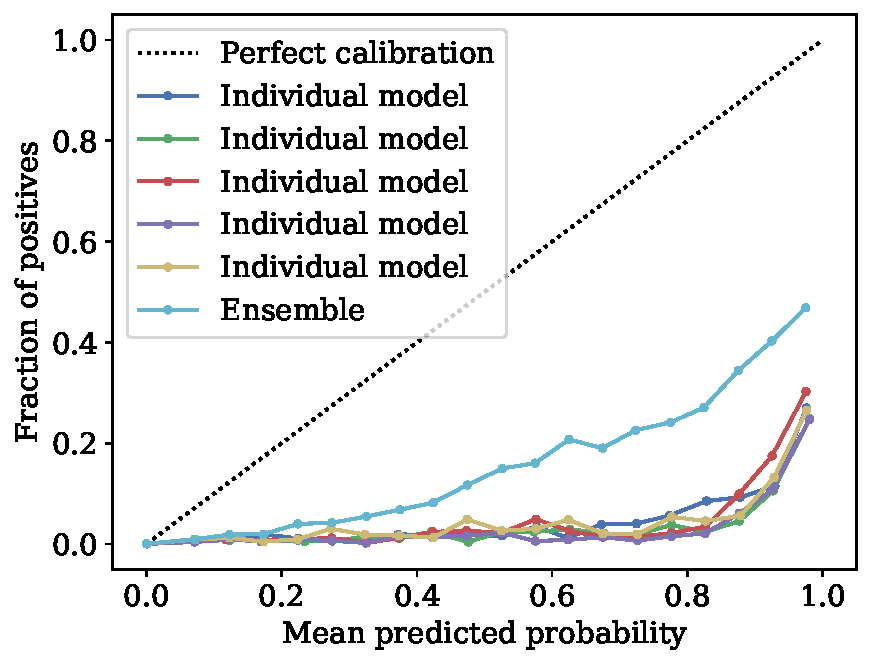
\includegraphics[width=1\columnwidth]{paper_retrospective_calibration_plots/calibration_curve_ensemble_and_all_models_uncalibrated.pdf}
        % \caption{}
        % \label{fig_discussion:calibration_curve_ensemble_and_all_models_uncalibrated}
    \end{subfigure}
    % \hfill
    \begin{subfigure}[c]{0.48\columnwidth}
        \centering
        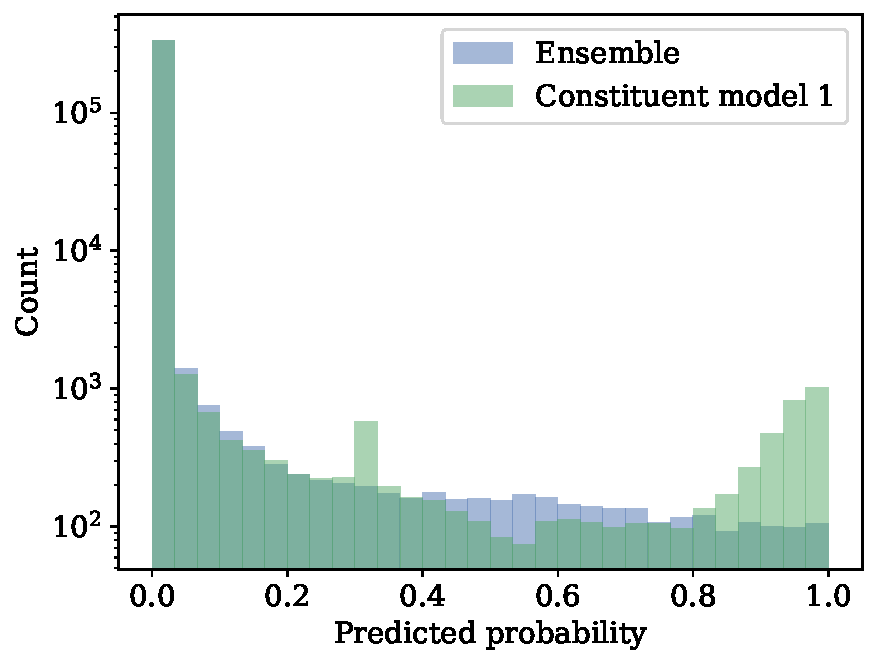
\includegraphics[width=1\columnwidth]{paper_retrospective_calibration_plots/histogram_ensemble_and_single_model.pdf}
        % \caption{}
        % \label{fig_discussion:histogram_ensemble_and_single_model}
    \end{subfigure}
    \caption[Calibration curve for the uncalibrated stroke recognition ensemble and empirical distribution of predicted probabilities.]{%
        Calibration curve for the uncalibrated stroke recognition ensemble (left) and the histogram of predicted probabilities (right) for the test set. 
        We use the ensemble that achieved the median F1-score reported in \cref{fig_retrospective:figure1-roc-curve} and \cref{tab_retrospective:table3-occlusion-analysis}.}
    \label{fig_discussion:retrospective-paper-calibration-curve-of-uncalibrated-model}
\end{figure}

Our work on stroke recognition in \cref{chp:paper-retrospective} focuses on the predictive performance of the ensemble model and an analysis of feature importance, but does not explicitly consider uncertainty estimation. 
As we discussed in \cref{subsec:model-calibration}, such a model can be calibrated to predict probabilities that are aligned with the empirical probability of the model being correct on some validation set. Here we present and discuss model calibration for the ensemble model. 

We compute the calibration curve by sorting the probabilities predicted on the test set into a number of bins spanning the range from zero to one. For each bin $b$, we compute the mean predicted probability $\bar{p}$ and the fraction of examples for which the model predicted correctly $r_{b}$. The calibration curve is the drawn from the $\{(\bar{p}_{b}, r_{b})\}_b$ pairs. For any given bin, a perfectly calibrated model would have the same fraction of correct predictions as that bin's mean value, $\bar{p}_{b} = r_{b}\,\forall\,b$. 

The calibration curve for the uncalibrated stroke recognition ensemble and its constituent models is plotted in \cref{fig_discussion:retrospective-paper-calibration-curve-of-uncalibrated-model} along with a histogram of its predicted probabilities. The miscalibration issue that we previously discussed is clearly visible as a strong overconfidence for both ensemble and constituents, although the ensemble is much better calibrated than its constituents. Since the ensemble's output probability is computed as the harmonic mean of the five constituent model probabilities, it can never exceed the maximum probability predicted between the constituent models. This property tends to make ensemble probabilities less extreme and, since the constituent models are overconfident, this results in better calibration (see also the histogram in \cref{fig_discussion:retrospective-paper-calibration-curve-of-uncalibrated-model}). 

\begin{figure}
    \centering
    \begin{subfigure}[c]{0.48\columnwidth}
        \centering
        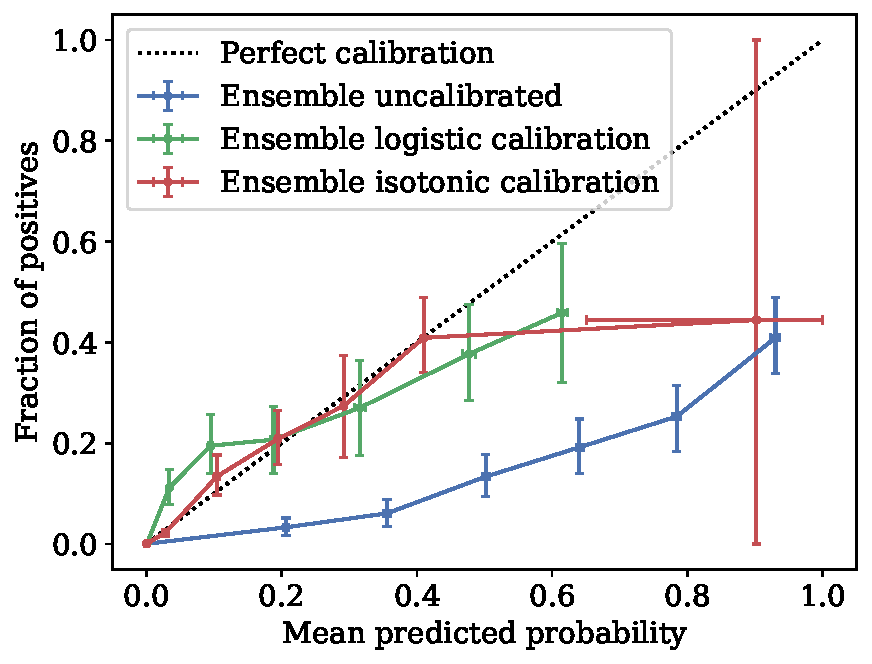
\includegraphics[width=1\columnwidth]{paper_retrospective_calibration_plots/calibration_curves_ensemble_with_cis.pdf}
    \end{subfigure}    
    \begin{subfigure}[c]{0.48\columnwidth}
        \centering
        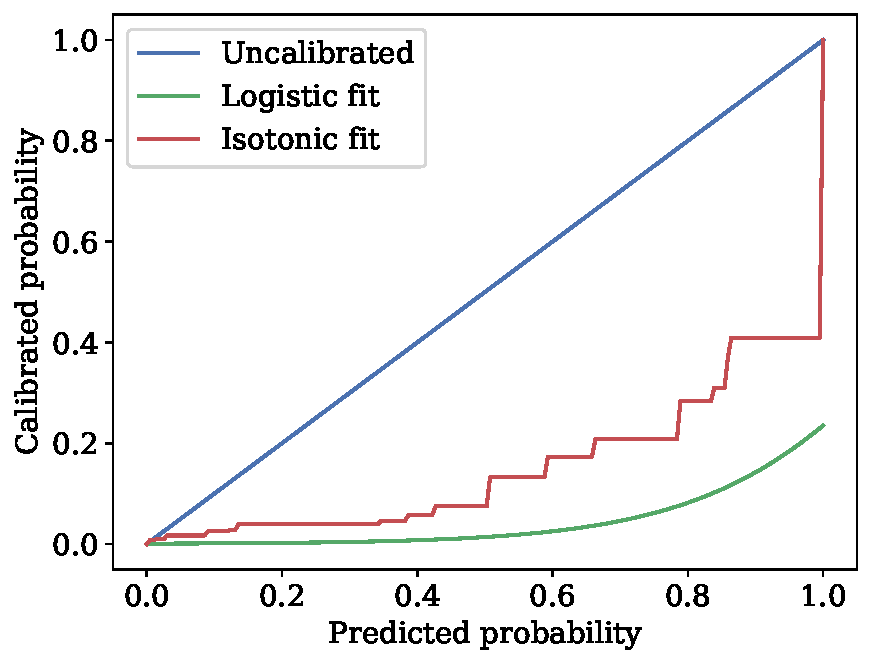
\includegraphics[width=1\columnwidth]{paper_retrospective_calibration_plots/calibration_fits_ensemble.pdf}
    \end{subfigure}    
    \caption[Calibration fits and curves for the stroke recognition ensemble using Platt-scaling and isotonic regression for calibration.]{ Calibration curves using sigmoid and isotonic calibration fits for the stroke recognition ensemble model (left) and the calibration fits (right) for the test set. We use the ensemble that achieved the median F1-score reported in \cref{fig_retrospective:figure1-roc-curve} and \cref{tab_retrospective:table3-occlusion-analysis}.}
    \label{fig_discussion:retrospective-paper-calibration-curve-sigmoid-isotonic}
\end{figure}
\begin{figure}
    \begin{subfigure}[c]{0.48\columnwidth}
        \centering
        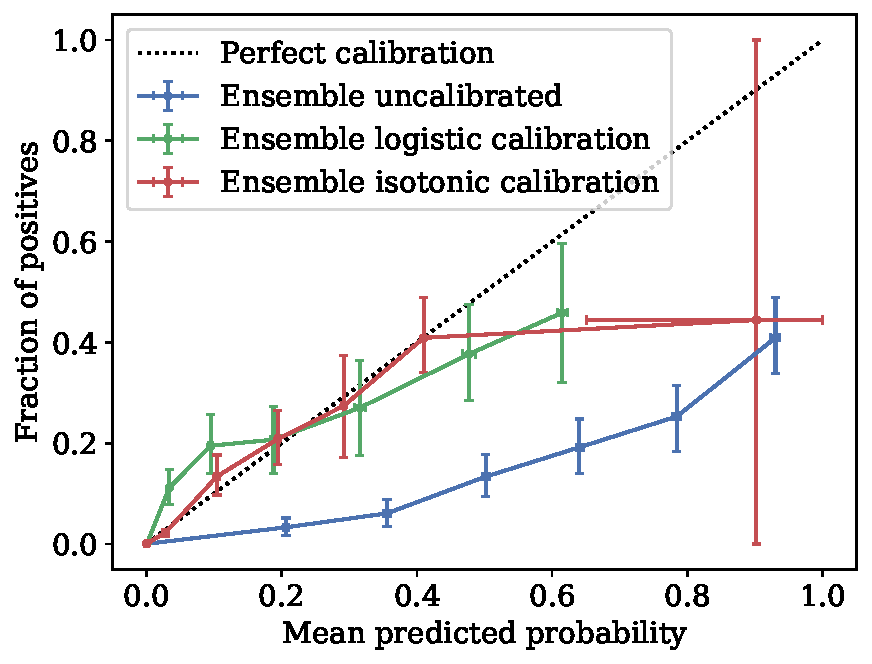
\includegraphics[width=1\columnwidth]{paper_retrospective_calibration_plots/calibration_curves_ensemble_with_cis.pdf}
    \end{subfigure}    
    \begin{subfigure}[c]{0.48\columnwidth}
        \centering
        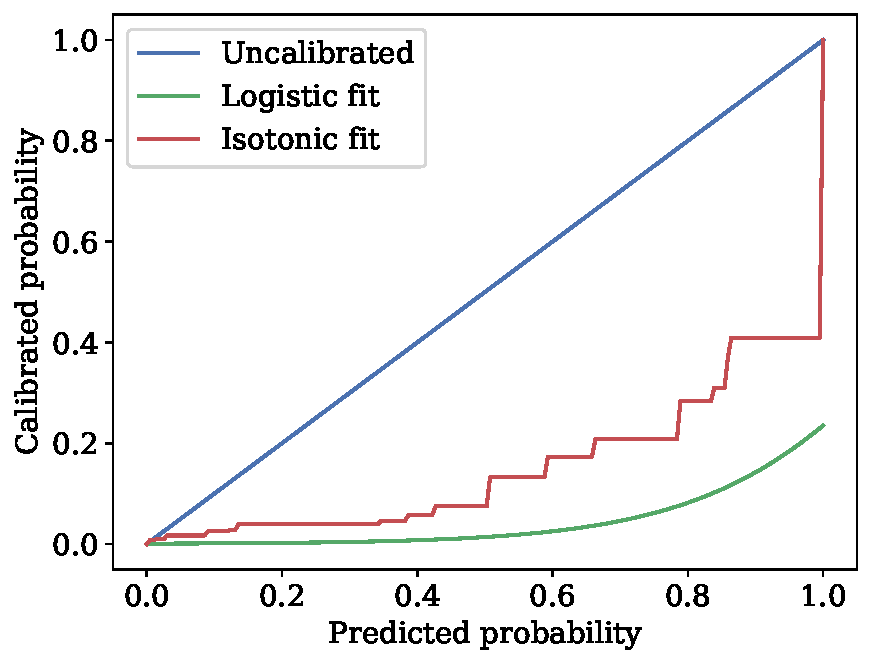
\includegraphics[width=1\columnwidth]{paper_retrospective_calibration_plots/calibration_fits_ensemble.pdf}
    \end{subfigure}    
    \caption[Calibration fits and curves for the stroke recognition ensemble using Platt-scaling and isotonic regression for calibration.]{ Calibration curves using sigmoid and isotonic calibration fits for the stroke recognition ensemble model (left) and the calibration fits (right) for the test set. We use the ensemble that achieved the median F1-score reported in \cref{fig_retrospective:figure1-roc-curve} and \cref{tab_retrospective:table3-occlusion-analysis}.}
    \label{fig_discussion:retrospective-paper-calibration-curve-sigmoid-isotonic}
\end{figure}    


To calibrate the ensemble model, we can use methods such as Platt-scaling \parencite{platt_probabilistic_1999} or isotonic regression \parencite{zadrozny_transforming_2002}. 
In either case, we fit a simple regression model (logistic or isotonic) to the predicted probabilities and the target labels on the validation set and use it to adjust the probabilities predicted on the test set. We show the resulting calibration curves on the left in \cref{fig_discussion:retrospective-paper-calibration-curve-sigmoid-isotonic} and the logistic and isotonic fits on the right with 95\% bootstrap confidence intervals on the bin centers ($x$ error) and fraction of positives ($y$ error). 
% In \cref{fig_discussion:retrospective-paper-calibration-curve-sigmoid-isotonic} we have done so for the ensemble model and visualize the results on the test set. 
% On the left, we plot the resulting calibration curves and on the right we show the logistic and isotonic fits. 
We see that both methods result in quite good calibrations\footnote{Brier scores on test set: Uncalibrated = $0.003500$, logistic = $0.001807$, isotonic = $0.001774$. Relative improvement in Brier score compared to uncalibrated (Brier skill score): Logistic = $0.4830$, isotonic = $0.4924$.} and that the predicted probabilities are shifted towards smaller values. 
Since stroke cases have low prevalence, high probability is predicted only for a few examples (see histogram in \cref{fig_discussion:retrospective-paper-calibration-curve-of-uncalibrated-model}). This leads to a lack of data for the calibration fits at high predicted probabilities which can be seen to result in poor generalization to the test set, especially for the nonparametric isotonic regression.

% Brier scores:  {'uncalibrated': 0.0034955788687128925, 'logistic': 0.0018072483306197486, 'isotonic': 0.0017744177396100578, 'average': 0.0021955477869598783}
% BSS uncalibrated reference:  {'logistic': 0.48299025755205005, 'isotonic': 0.4923822902432705}
% BSS mean reference:  {'logistic': 0.17685766561145932, 'isotonic': 0.1918109229282361}

\begin{figure}
    % \begin{subfigure}[c]{0.48\columnwidth}
    %     \centering
    %     \includegraphics[width=1\columnwidth]{paper_retrospective_calibration_plots/precision_vs_predicted_probability_ensemble_calltaker_with_cis.pdf}
    %     % \caption{}
    %     % \label{fig_discussion:calibration_curve_ensemble_and_all_models_uncalibrated}
    % \end{subfigure}    
    % % \hfill
    % \begin{subfigure}[c]{0.48\columnwidth}
    %     \centering
    %     \includegraphics[width=1\columnwidth]{paper_retrospective_calibration_plots/recall_vs_predicted_probability_ensemble_calltaker_with_cis.pdf}
    %     % \caption{}
    %     % \label{fig_discussion:histogram_ensemble_and_single_model}
    % \end{subfigure}
    \begin{subfigure}[c]{0.48\columnwidth}
        \centering
        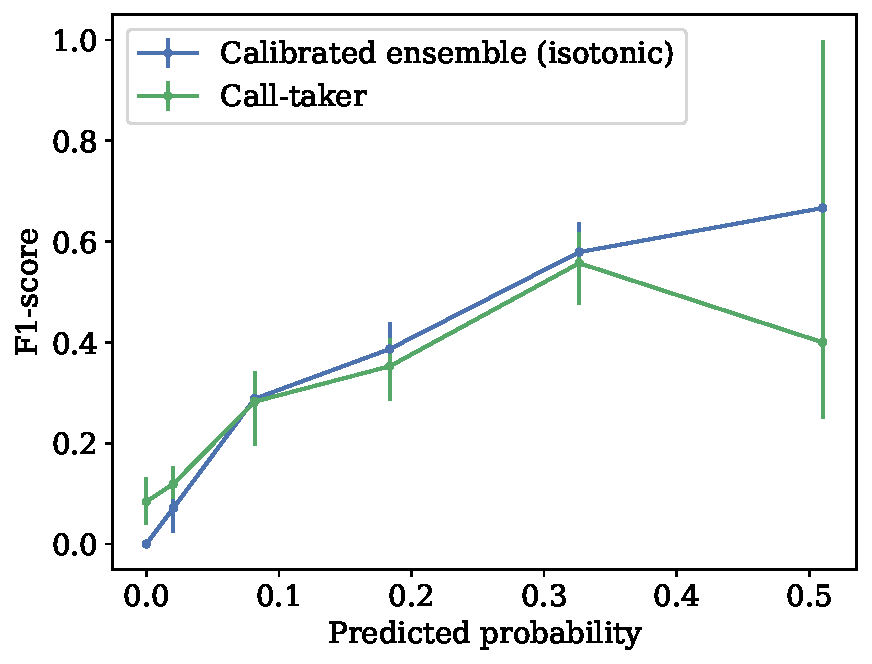
\includegraphics[width=1\columnwidth]{paper_retrospective_calibration_plots/f1_score_vs_predicted_probability_ensemble_calltaker_with_cis.pdf}
    \end{subfigure}    
    \begin{subfigure}[c]{0.48\columnwidth}
        \centering
        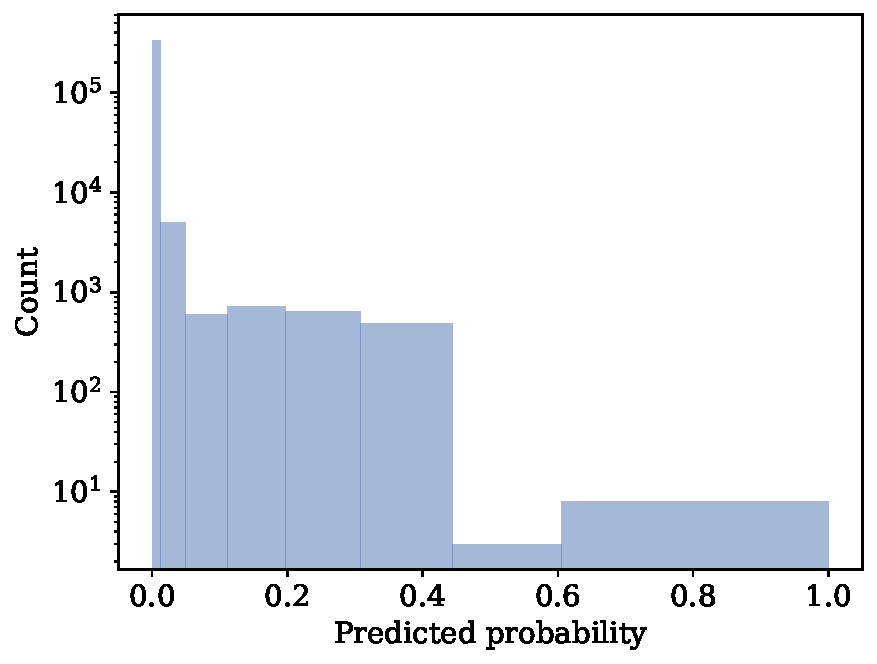
\includegraphics[width=1\columnwidth]{paper_retrospective_calibration_plots/predicted_probability_histogram.pdf}
    \end{subfigure}    
    \caption[Comparison of F1-score of stroke recognition ensemble and call-takers as function of predicted probability.]{ Comparison of the F1-score of the stroke recognition ensemble and call-takers. The F1-score is computed on subsets of the test dataset made by binning on the predicted probabilities of the calibrated ensemble. We see that the relative performance improvement of the ensemble over call-takers is higher towards more certain predictions. We use the ensemble that achieved the median F1-score reported in \cref{fig_retrospective:figure1-roc-curve} and \cref{tab_retrospective:table3-occlusion-analysis}.}
    \label{fig_discussion:retrospective-paper-f1-performance-vs-predicted-probability}
\end{figure}

Clinicians in intensive care units and emergency departments have been found to strongly agree that a singular focus on overall accuracy cannot alone ensure sustained trust in a model \cite{tonekaboni_what_2019}. Clinicians expect an alert to present a prediction that aligns with patient status. Despite expert-agreed thresholds for when alerts should be triggered, however, many alerts may not be aligned since the unbalanced and ambiguous nature of many predictive problems in healthcare can lead to relatively low predictive precision \parencite{umscheid_development_2015, cite14, cite15, wenstrup_retrospective_2023}. This is likely to lead to alarm fatigue \parencite{embi_evaluating_2012} and can undermine the sustained use and endorsement by clinicians of such systems \parencite{guidi_clinician_2015}. 
The expected precision of the stroke recognition ensemble presented in \cref{chp:paper-retrospective} is $24.9\%$ (95\% confidence interval $24.3-25.5\%)$. This bluntly means it might be wrong three out of four times it predicts a positive. This unfortunately risks alarm fatigue among its potential users which might diminish it's real-world impact.

% If the stroke recognition ensemble were to be deployed in a randomized controlled trial, s
Such issues might be alleviated by incorporating the calibrated probabilities in the alerts presented to users. Presented with calibrated probabilities, users would be able to discern between certain and uncertain predictions. Furthermore, calibrated probabilities might be used to present users only with predictions that exceed a specific confidence level. Similar approaches have been suggested by clinicians and interviews indicate that predictive uncertainty is perceived as a sort of explanation that complements the prediction \cite{tonekaboni_what_2019}. In \cref{fig_discussion:retrospective-paper-f1-performance-vs-predicted-probability} we show the F1-score of the ensemble model and the call-takers computed on subsets of the data created by binning the predicted probilities of the isotonically calibrated ensemble. We note that as might be expected, both call-taker and ensemble model performance increase with increased model certainty. This indicates that selecting, based on certainty, which predictions to present to users might indeed help improve trust in the system in practice. 


% \lesstodo[inline]{Maybe mention MultiQT paper \parencite{havtorn_multiqt_2020}.}
